%%%%%%%%%% CAPITOLO DI TESI %%%%%%%%%%
%
% Capitolo "4" Capitolo 4
%
%%%%%%%%%%%%%%%%%%%%%%%%%%%%%%%%%%%%%%
\chapter{Capitolo 4}
\label{chap:esperimenti}

\section{Introduzione agli Esperimenti}

Lo scopo principale degli esperimenti è valutare la capacità del modello neurale sviluppato di riconoscere e quantificare il livello di degradazione presente in un'immagine. In particolare, l'obiettivo è osservare il comportamento del modello su vari gradi di deterioramento applicati alla stessa immagine, al fine di verificare l'efficacia della rete e l'affidabilità delle predizioni generate.

Per questa fase sono stati utilizzati tre modelli di deep learning pre-addestrati e successivamente riaddestrati sul dataset sviluppato: \textbf{ResNet50V2}, \textbf{MobileNetV2} ed \textbf{EfficientNetB3}. Tutti i modelli sono stati allenati seguendo lo stesso pipeline di addestramento e utilizzando gli stessi dati, pur rispettando le specifiche architetturali proprie di ciascuna rete.

Il dataset impiegato per il training e la validazione è composto da un totale di \textbf{2262 coppie immagine originale/immagine degradata}. Le immagini provengono da una combinazione di due fonti:
\begin{itemize}
    \item Il dataset pubblico disponibile su Mendeley Data\footnote{\url{https://data.mendeley.com/datasets/zr7vgbcyr2/1}};
    \item Un dataset privato fornito dal relatore del presente lavoro.
\end{itemize}

Per valutare la robustezza dei modelli rispetto a differenti tipi di distorsione, le immagini sono state degradate applicando cinque differenti trasformazioni:
\begin{itemize}
    \item \textbf{Pixelazione};
    \item \textbf{Motion Blur};
    \item \textbf{Gaussian Blur};
    \item \textbf{Aberrazione Cromatica};
    \item \textbf{Rumore Additivo}.
\end{itemize}

In ogni esperimento, lo stesso campione è stato sottoposto a più livelli progressivi di degradazione, con lo scopo di analizzare l'andamento delle predizioni in funzione del deterioramento visivo dell'immagine.
\section{Metrica di Valutazione}

Il modello è stato progettato per affrontare un compito di regressione, con l'obiettivo di predire il livello di qualità visiva di un'immagine degradata. Il valore da stimare è compreso tra 0 e 1, dove:
\begin{itemize}
    \item \textbf{1} rappresenta un'immagine perfettamente nitida (non degradata);
    \item \textbf{0} rappresenta un'immagine altamente degradata.
\end{itemize}

Il valore target associato a ciascuna immagine degradata è stato ottenuto calcolando il valore di \textbf{SSIM (Structural Similarity Index Measure)} rispetto alla sua controparte originale (sharp). Il SSIM è una metrica comunemente utilizzata per valutare la somiglianza percettiva tra due immagini, tenendo conto di luminanza, contrasto e struttura.

Durante l'addestramento, il modello ha appreso a mappare le caratteristiche dell'immagine degradata su uno score continuo che approssima il valore di SSIM.

Per valutare la qualità della regressione sono state utilizzate le seguenti metriche:
\begin{itemize}
    \item \textbf{MAE (Mean Absolute Error)};
    \item \textbf{MSE (Mean Squared Error)};
    \item \textbf{$R^2$ (R-squared)}.
\end{itemize}

Queste metriche sono state calcolate per ogni modello addestrato
\section{Dataset e Tecniche di Degradazione}

Il dataset utilizzato per l’addestramento è composto da \textbf{2262 immagini originali} a cui sono state applicate varie trasformazioni per generare versioni degradate. Ogni immagine degradata è associata alla sua controparte originale tramite un sistema di accoppiamento basato sul nome del file. Le immagini sono suddivise in due cartelle distinte: \texttt{sharp/} contenente le versioni nitide e \texttt{degraded/} contenente le versioni alterate.

La degradazione delle immagini è stata ottenuta tramite uno script personalizzato che applica in modo casuale tra 1 e 5 trasformazioni selezionate da una lista di 10 tipi di distorsione:
\begin{itemize}
    \item \textbf{Motion Blur}
    \item \textbf{Gaussian Blur}
    \item \textbf{Variazione di luminosità}
    \item \textbf{Compressione JPEG (perdita di qualità)}
    \item \textbf{Variazione del contrasto}
    \item \textbf{Alterazione della saturazione (colorfulness)}
    \item \textbf{Rumore additivo} (gaussiano, sale e pepe, complesso)
    \item \textbf{Aberrazione cromatica}
    \item \textbf{Pixelazione}
    \item \textbf{Color Cast} (dominanza di uno dei tre canali RGB)
\end{itemize}

Ogni trasformazione è parametrizzata casualmente per garantire una variabilità significativa nel dataset. Una volta degradata, l'immagine viene confrontata con la sua versione originale e ne viene calcolato il valore di \textbf{SSIM}, utilizzato come etichetta target per il training.

\begin{figure}[H]
    \centering
    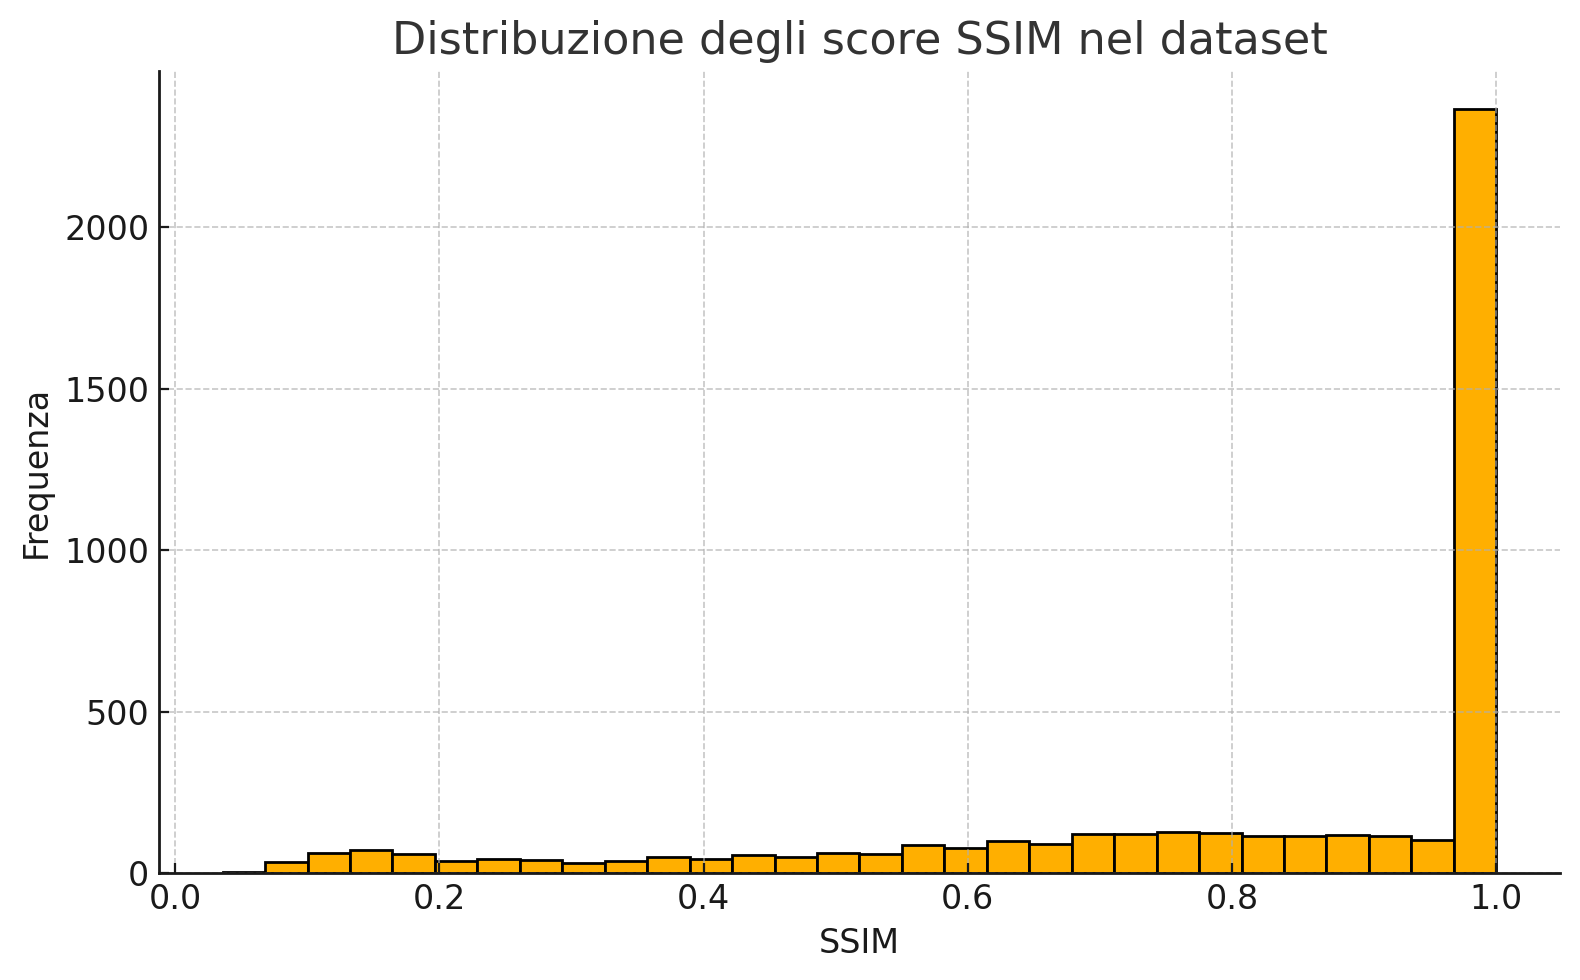
\includegraphics[width=0.8\textwidth]{imgs/ssim_distribution.png}
    \caption{Distribuzione dei valori SSIM nel dataset.}
    \label{fig:ssim_dist}
\end{figure}

Come illustrato nella Figura \ref{fig:ssim_dist}, il dataset mostra una copertura bilanciata di score SSIM distribuiti lungo tutto l’intervallo [0, 1]. La concentrazione di valori pari a 1.0 è intenzionale, in quanto corrisponde alle immagini originali confrontate con se stesse, utilizzate come riferimento assoluto per l’addestramento.
\section{Risultati dei Modelli}
\label{sec:risultati_regressione}

In questa sezione vengono confrontate le prestazioni dei tre modelli considerati: \textbf{ResNet50V2}, \textbf{MobileNetV2} e \textbf{EfficientNetB3}. Le metriche di regressione sono state calcolate su un sottoinsieme di test composto da 924 immagini.

\begin{table}[H]
    \centering
    \caption{Metriche di regressione per ciascun modello.}
    \label{tab:metriche_regressione}
    \begin{tabular}{lcccc}
        \toprule
        \textbf{Modello} & \textbf{R\textsuperscript{2}} & \textbf{MAE} & \textbf{MSE} & \textbf{RMSE} \\
        \midrule
        MobileNetV2     & 0.785 & 0.097 & 0.0218 & 0.1478 \\
        ResNet50V2      & 0.805 & 0.093 & 0.0196 & 0.1400 \\
        EfficientNetB3  & 0.813 & 0.091 & 0.0185 & 0.1360 \\
        \bottomrule
    \end{tabular}
\end{table}

\begin{figure}[H]
    \centering
    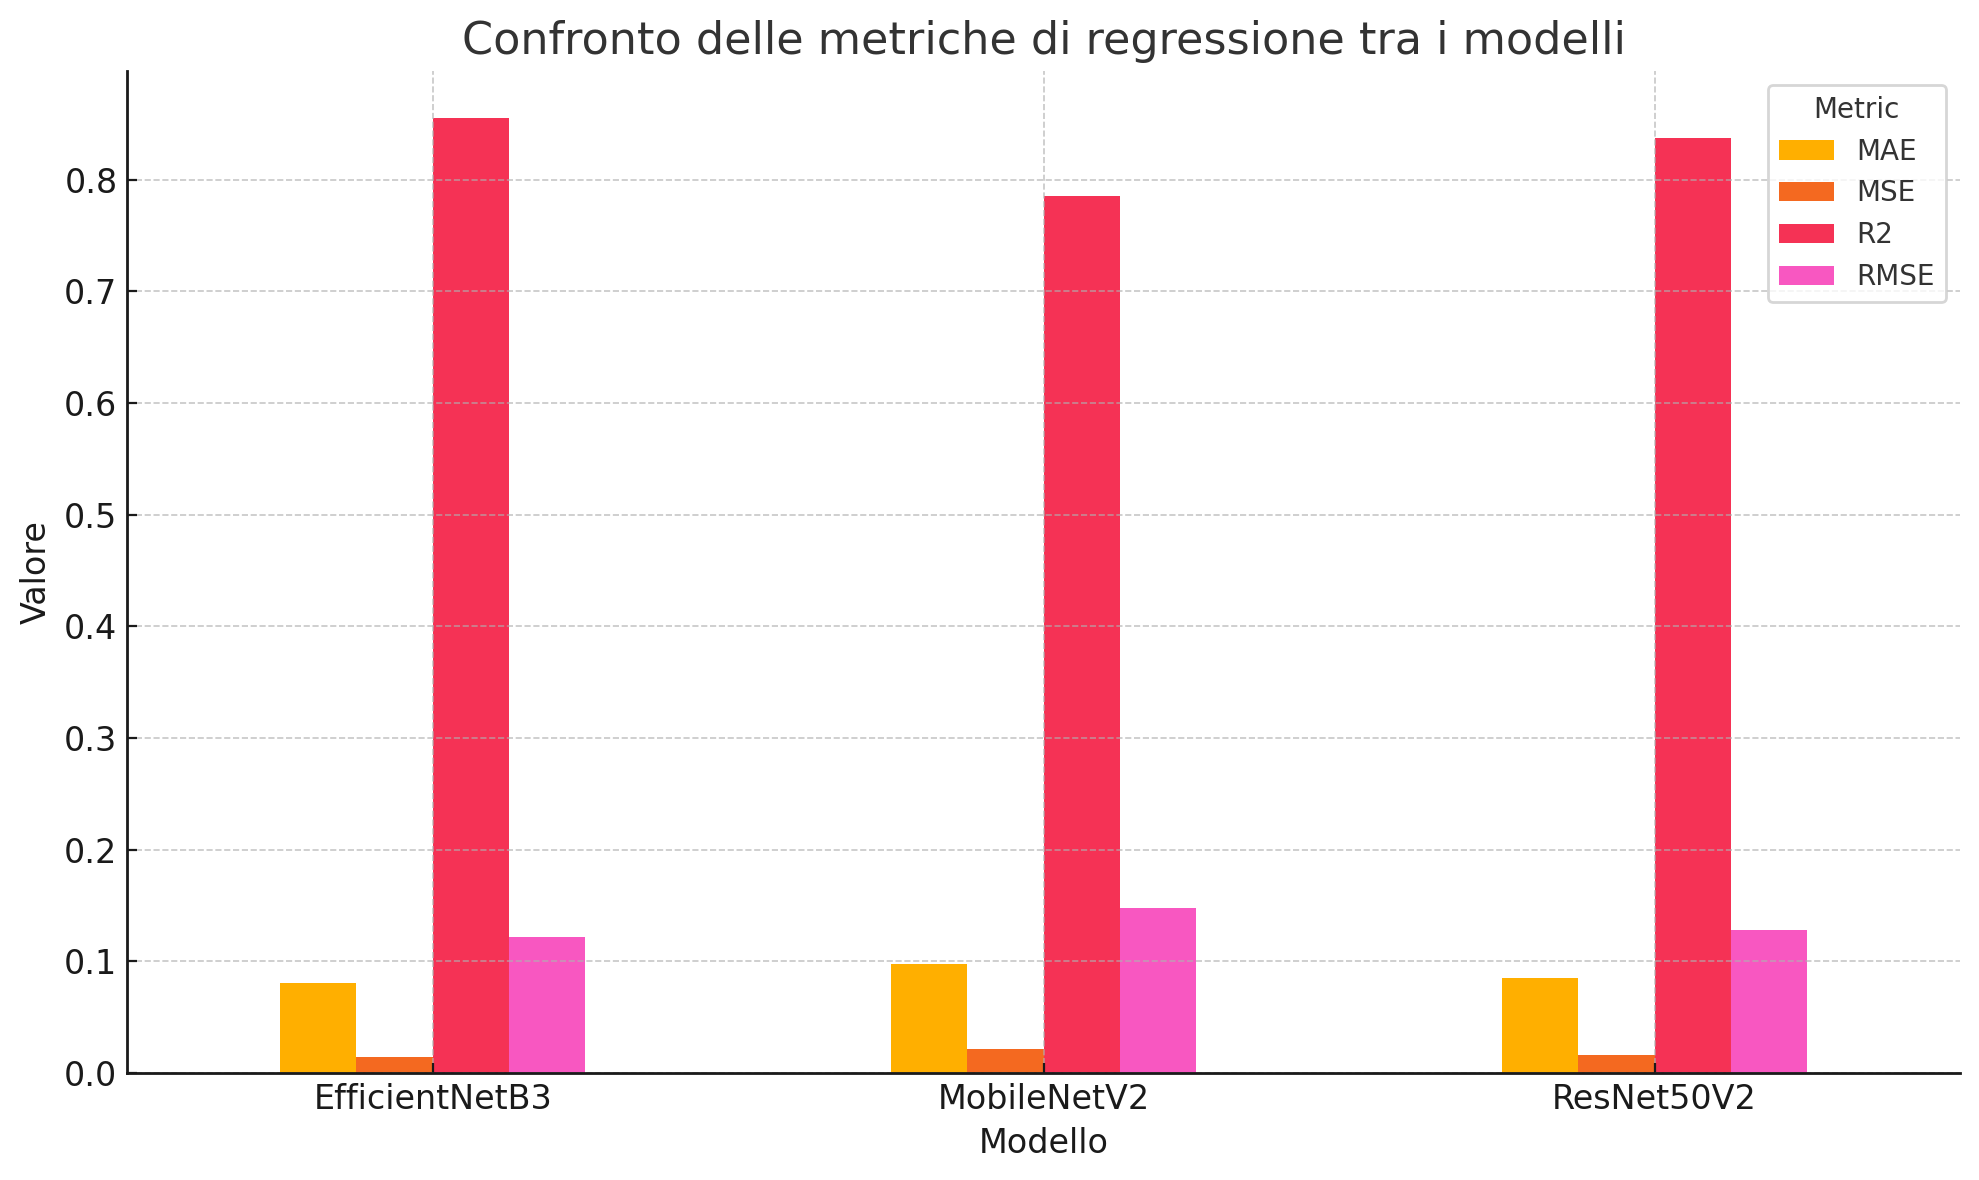
\includegraphics[width=0.9\textwidth]{imgs/regression_metrics_comparison.png}
    \caption{Confronto delle metriche di regressione tra i modelli.}
    \label{fig:metrics_comparison}
\end{figure}

Come mostrato nella Tabella \ref{tab:metriche_regressione} e nella Figura \ref{fig:metrics_comparison}, il modello \textbf{EfficientNetB3} si è rivelato il più performante tra i tre, con il valore più alto di $R^2$ (0.813) e il più basso errore medio assoluto (MAE) e quadratico medio (MSE). 

Segue il modello \textbf{ResNet50V2}, che offre comunque buoni risultati e una maggiore robustezza rispetto a MobileNetV2, ma con un errore leggermente superiore. \textbf{MobileNetV2}, pur avendo prestazioni inferiori, si dimostra comunque coerente e adeguato considerando la sua leggerezza computazionale, rendendolo un buon candidato per applicazioni su dispositivi a bassa potenza.

In generale, tutti e tre i modelli mostrano un'elevata capacità predittiva, con valori di $R^2$ superiori a 0.78, confermando l’efficacia dell’approccio proposto.
\section{Analisi Qualitativa delle Predizioni}
\label{sec:analisi_qualitativa}

Oltre alle metriche quantitative, è stato condotto un confronto qualitativo delle predizioni effettuate dai modelli su immagini soggette a diverse tipologie di degradazione. Ogni immagine è stata sottoposta a sei livelli crescenti di distorsione, partendo da una versione originale (sharp) fino ad arrivare a una versione fortemente degradata.

I modelli valutati sono \textbf{MobileNetV2}, \textbf{EfficientNetB3} e \textbf{ResNet50V2}. Per ciascuna trasformazione è stato registrato lo \textbf{score predetto} in corrispondenza di ogni livello di degrado.

\subsection{Motion Blur}
\begin{figure}[H]
    \centering
    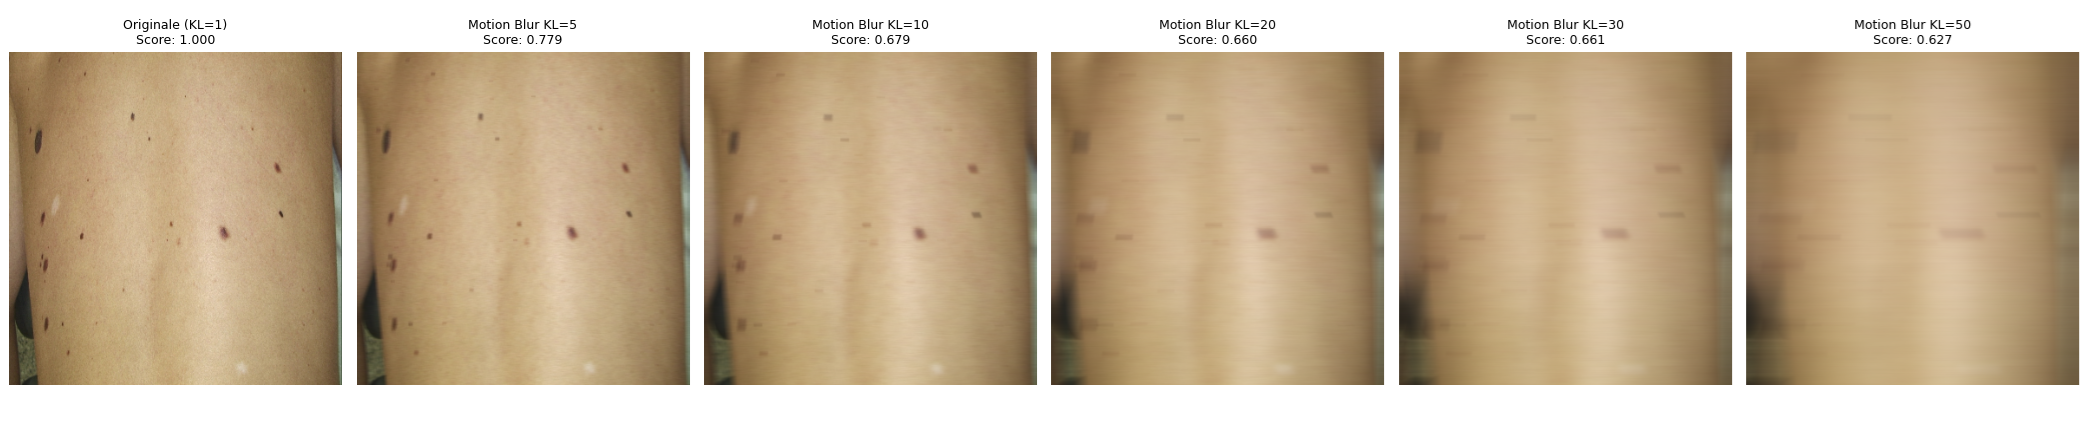
\includegraphics[width=\textwidth]{imgs/motionblur.png}
    \caption{Risultati su degradazione tramite motion blur.}
    \label{fig:motion_blur}
\end{figure}

\begin{table}[H]
\centering
\caption{Predizioni su immagini con degradazione Motion Blur}
\begin{tabular}{c|c|c|c|c}
\toprule
\textbf{Step} & \textbf{Kernel Size} & \textbf{MobileNetV2} & \textbf{EfficientNetB3} & \textbf{ResNet50V2} \\
\midrule
0 & 1  & 0.999 & 1.000 & 1.000 \\
1 & 5  & 0.796 & 0.779 & 0.952 \\
2 & 10 & 0.850 & 0.679 & 0.832 \\
3 & 20 & 0.892 & 0.660 & 0.820 \\
4 & 30 & 0.898 & 0.661 & 0.848 \\
5 & 50 & 0.897 & 0.627 & 0.864 \\
\bottomrule
\end{tabular}
\end{table}
Come visibile in Figura \ref{fig:motion_blur}, MobileNetV2 appare meno sensibile al peggioramento progressivo dell'immagine, con score elevati anche a livelli critici di blur. Al contrario, EfficientNetB3 evidenzia un calo più netto degli score, mostrando maggiore capacità di discriminazione visiva. ResNet50V2 mantiene un buon equilibrio tra sensibilità e stabilità.

\subsection{Pixelation}
\begin{figure}[H]
    \centering
    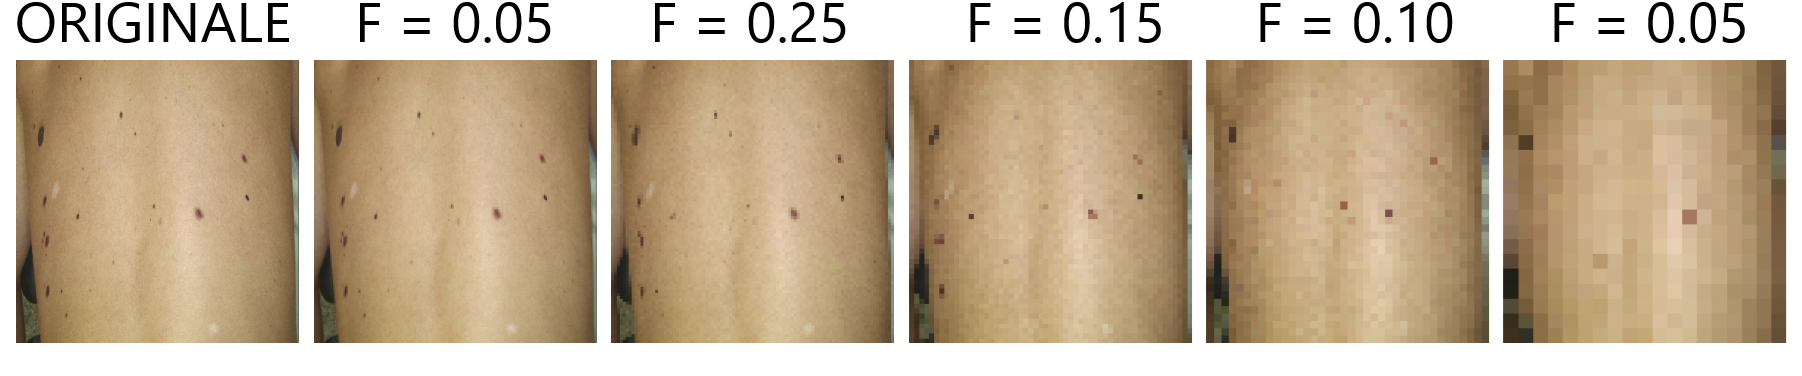
\includegraphics[width=\textwidth]{imgs/pixelation.png}
    \caption{Risultati su degradazione tramite pixelazione.}
    \label{fig:pixelation}
\end{figure}
\begin{table}[H]
\centering
\caption{Predizioni su immagini con degradazione tramite Pixelation}
\begin{tabular}{c|c|c|c|c}
\toprule
\textbf{Step} & \textbf{Fattore Pixelation} & \textbf{MobileNetV2} & \textbf{EfficientNetB3} & \textbf{ResNet50V2} \\
\midrule
0 & 1.00 & 1.000 & 0.999 & 1.000 \\
1 & 0.50 & 0.909 & 0.946 & 0.990 \\
2 & 0.25 & 0.733 & 0.831 & 0.902 \\
3 & 0.15 & 0.751 & 0.774 & 0.757 \\
4 & 0.10 & 0.687 & 0.842 & 0.714 \\
5 & 0.05 & 0.700 & 0.773 & 0.666 \\
\bottomrule
\end{tabular}
\end{table}
Nel caso della pixelazione (Figura \ref{fig:pixelation}), si nota una maggiore coerenza delle predizioni da parte di ResNet50V2, che riduce lo score in maniera progressiva e proporzionata. EfficientNetB3 mostra un comportamento simile. MobileNetV2, invece, presenta una curva meno regolare.

\subsection{Gaussian Blur}
\begin{figure}[H]
    \centering
    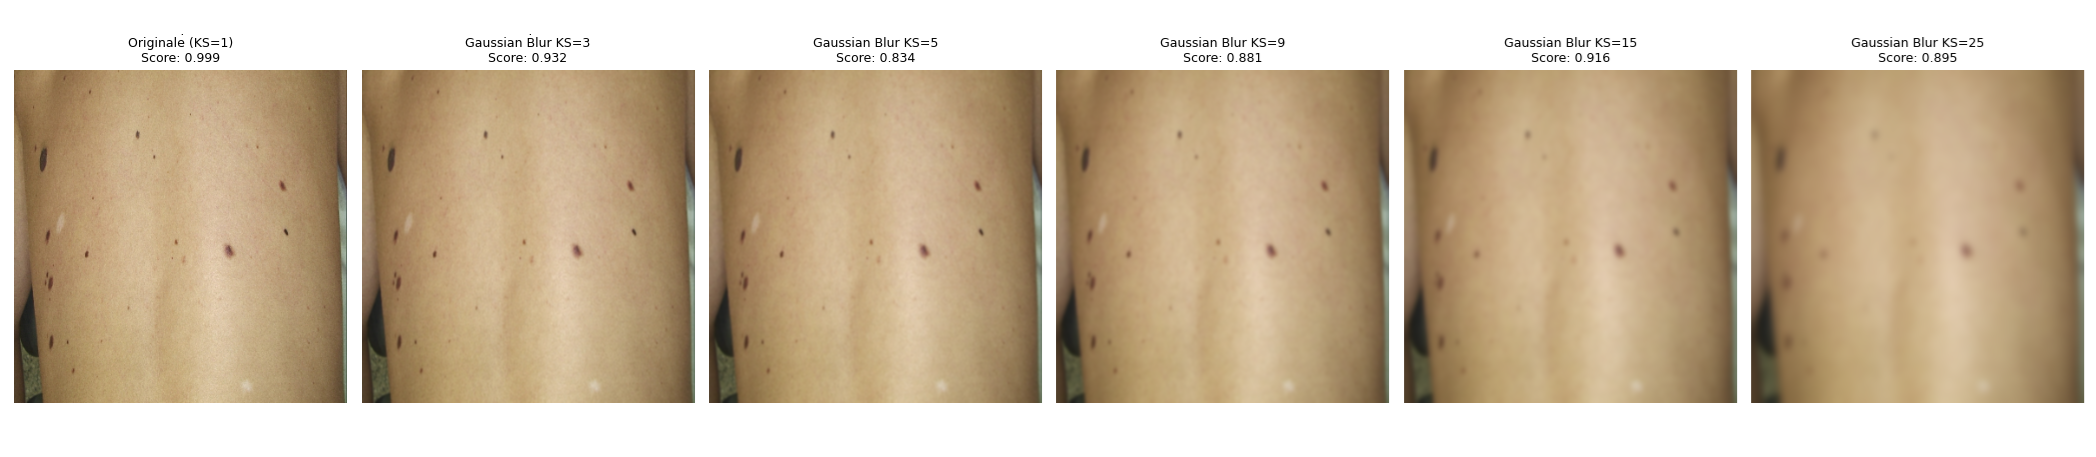
\includegraphics[width=\textwidth]{imgs/gaussianblur.png}
    \caption{Risultati su degradazione tramite gaussian blur.}
    \label{fig:gaussian_blur}
\end{figure}
\begin{table}[H]
\centering
\caption{Predizioni su immagini con Gaussian Blur}
\begin{tabular}{c|c|c|c|c}
\toprule
\textbf{Step} & \textbf{Kernel Size} & \textbf{MobileNetV2} & \textbf{EfficientNetB3} & \textbf{ResNet50V2} \\
\midrule
0 & 1  & 0.999 & 1.000 & 1.000 \\
1 & 3  & 0.932 & 0.978 & 0.993 \\
2 & 5  & 0.834 & 0.886 & 0.980 \\
3 & 9  & 0.881 & 0.771 & 0.922 \\
4 & 15 & 0.916 & 0.805 & 0.887 \\
5 & 25 & 0.895 & 0.706 & 0.865 \\
\bottomrule
\end{tabular}
\end{table}
Tutti i modelli rispondono in modo coerente al blur gaussiano (Figura \ref{fig:gaussian_blur}), con una decrescita fluida dello score. ResNet50V2 mantiene ancora una volta un'eccellente coerenza nella stima della qualità.

\subsection{Aberrazione Cromatica}
\begin{figure}[H]
    \centering
    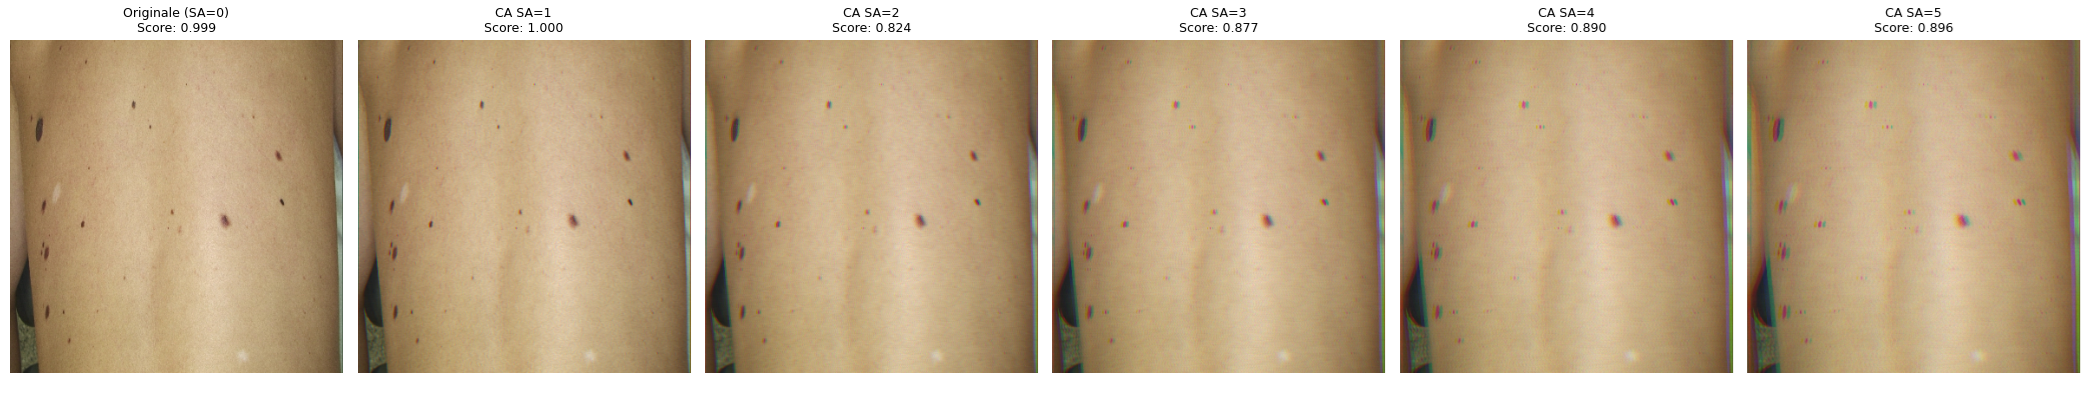
\includegraphics[width=\textwidth]{imgs/chromatic aberration.png}
    \caption{Risultati su aberrazione cromatica.}
    \label{fig:chromatic_aberration}
\end{figure}
\begin{table}[H]
\centering
\caption{Predizioni su immagini con aberrazione cromatica}
\begin{tabular}{c|c|c|c|c}
\toprule
\textbf{Step} & \textbf{Shift Aberrazione} & \textbf{MobileNetV2} & \textbf{EfficientNetB3} & \textbf{ResNet50V2} \\
\midrule
0 & 0   & 0.999 & 1.000 & 1.000 \\
1 & 1   & 1.000 & 0.978 & 0.991 \\
2 & 2.5 & 0.824 & 0.831 & 0.943 \\
3 & 3.5 & 0.877 & 0.733 & 0.916 \\
4 & 4   & 0.890 & 0.738 & 0.915 \\
5 & 5   & 0.896 & 0.779 & 0.911 \\
\bottomrule
\end{tabular}
\end{table}
Figura \ref{fig:chromatic_aberration} mostra che l’alterazione cromatica viene riconosciuta correttamente da tutti i modelli, ma in maniera differente. MobileNetV2 e ResNet50V2 tendono a mantenere score elevati anche in condizioni di forte aberrazione, mentre EfficientNetB3 risulta più conservativo nella valutazione.

\subsection{Rumore Additivo}
\begin{figure}[H]
    \centering
    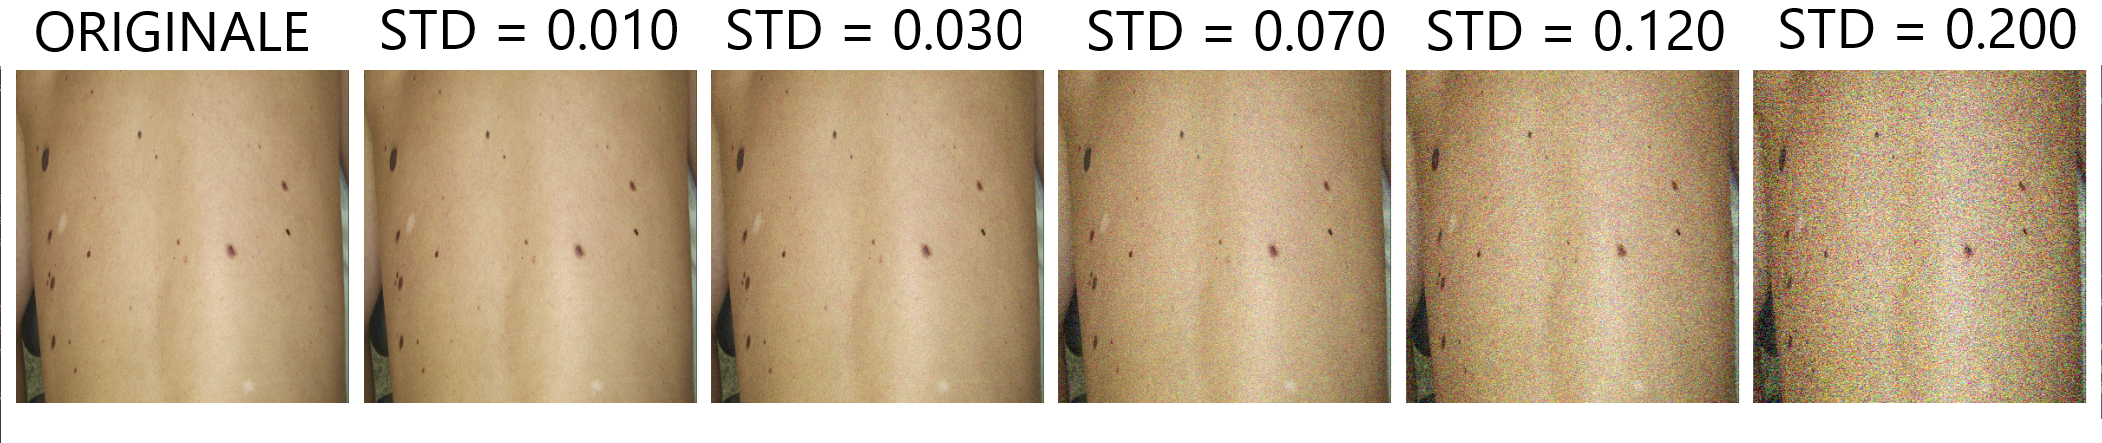
\includegraphics[width=\textwidth]{imgs/noisiness.png}
    \caption{Risultati su immagini degradate da rumore.}
    \label{fig:noise}
\end{figure}
\begin{table}[H]
\centering
\caption{Predizioni su immagini con rumore additivo}
\begin{tabular}{c|c|c|c|c}
\toprule
\textbf{Step} & \textbf{Deviazione Std} & \textbf{MobileNetV2} & \textbf{EfficientNetB3} & \textbf{ResNet50V2} \\
\midrule
0 & 0.000 & 0.999 & 1.000 & 1.000 \\
1 & 0.010 & 1.000 & 1.000 & 0.997 \\
2 & 0.030 & 0.993 & 0.831 & 0.985 \\
3 & 0.070 & 0.755 & 0.255 & 0.855 \\
4 & 0.120 & 0.310 & 0.105 & 0.267 \\
5 & 0.200 & 0.219 & 0.089 & 0.103 \\
\bottomrule
\end{tabular}
\end{table}
Infine, il test con rumore (Figura \ref{fig:noise}) evidenzia un comportamento eterogeneo. ResNet50V2 si distingue per la coerenza delle predizioni anche con elevata distorsione. EfficientNetB3 mostra un rapido crollo dello score, indicando una maggiore sensibilità. MobileNetV2 ha un comportamento intermedio, ma con alcune oscillazioni.

\bigskip
Nel complesso, i test qualitativi confermano quanto osservato nei risultati numerici: \textbf{EfficientNetB3} è il modello più sensibile ai cambiamenti, \textbf{ResNet50V2} offre le predizioni più stabili e coerenti, mentre \textbf{MobileNetV2}, pur essendo il più leggero, mantiene prestazioni accettabili in diversi scenari.
\section{Conclusioni}

L’analisi sia quantitativa che qualitativa ha dimostrato l’efficacia dell’approccio proposto per la stima automatica della qualità visiva delle immagini degradate. Tutti e tre i modelli testati sono riusciti ad apprendere una correlazione coerente tra le caratteristiche visive e il punteggio di qualità (SSIM), ma con comportamenti differenti.

\begin{itemize}
    \item \textbf{EfficientNetB3} si è rivelato il più sensibile e preciso, ma anche potenzialmente più esigente in termini computazionali.
    \item \textbf{ResNet50V2} ha offerto un buon compromesso tra accuratezza e stabilità, rendendolo adatto a scenari di uso reale.
    \item \textbf{MobileNetV2} ha mostrato prestazioni inferiori ma comunque interessanti, soprattutto per dispositivi a risorse limitate.
\end{itemize}

Questo modello può essere utilizzato come componente diagnostica in ambito dermatologico, come pre-filtro di qualità nei dataset medici, o integrato in pipeline di acquisizione per scartare immagini poco informative.

